\section{Results}
%Below we describe the results in the same order the experiments were described, first validating the adaptive momentum effect, then moving onto benchmarking and replay experiment results.  

\begin{figure*}[h!]
\begin{center}
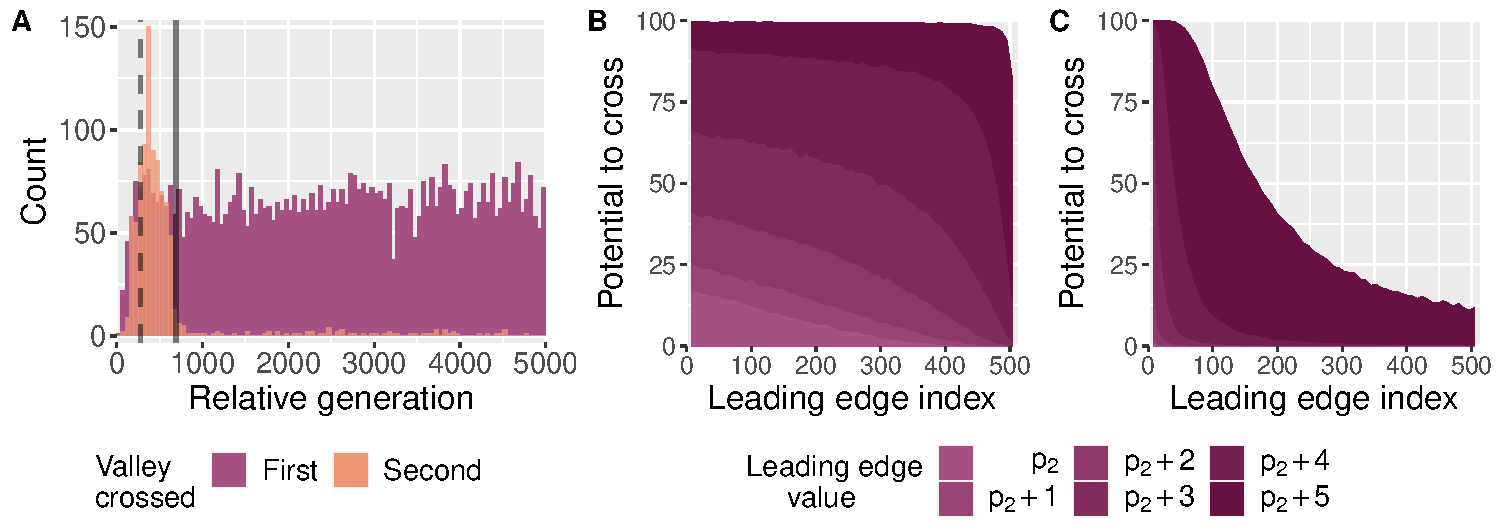
\includegraphics[width=\textwidth]{05_adaptive_momentum/media/combined_plots_full_split.pdf}
\caption{
    (A)
    Distribution of the number of generations required to cross valleys in the validation experiment. 
    Relative generations refer to the elapsed time (in generations) for the first cross (purple), and from the first cross to the second cross (orange). 
    %The solid and dashed horizontal lines show the expected count of first and second crosses per bar, respectively, for the expected uniform distribution. 
    The dashed and solid vertical lines show minimum and maximum fixation times, respectively. 
    (B) 
    Benchmarking data showing the potential of a leading edge to cross a valley, with a range of leading edge starting positions and values (see Fig. \ref{fig-experiment2}). 
    Each point represents 10,000 replicates.
    (C)
    Shuffled benchmarking data. Each replicate is shuffled prior to evolution, otherwise identical to center plot.
}
\label{fig-combined-plots}
\end{center}
\end{figure*}

\subsection{Validation of adaptive momentum effect}

First, we measured the time it took for replicates starting from a full population of $p_{2}$ to cross the valley to $p_{3}$ and, when relevant, from $p_{3}$ to $p_{4}$.
Figure \ref{fig-combined-plots}A
shows the timing distributions of populations that crossed the first valley over the first 5,000 generations (purple) as well as the timing distributions of second crossings that occur within 5,000 generations of a first (orange). 
We see that the time of first crossing appear uniformly distributed across the 5,000 generations, while the second crosses are strongly skewed toward shorter time periods. 
Indeed, of 500,000 replicates, 6,485 crossed the first valley within 5,000 generations (\localapprox 1.3\%) with a mean cross time of \localapprox 2,569 generations and a median of 2,602 generations. 
Based on these values, we would expect roughly 84 replicates to cross twice ($6,485 \times 1.3\%$, or 0.0169\% of all 500,000 replicates), but instead we see 902 replicates (\localapprox 0.18\%) cross the second valley, a much higher rate than expected if the probabilities of first and second crossing were equal.
In addition to a higher than expected rate of crossing, the mean cross time between first and second crossings is \localapprox 579 generations and the median cross time is 401 generations, substantially lower than the first crossing times. 
Finally, when we consider only those second crossing times that occurred more than 1000 generations after a first crossing, we find that the rate of these second crossings is similar to the first crossing rate (\localapprox 1.23\%).
These results comport with the framework of adaptive momentum. 
They show that an initial beneficial discovery can quickly lead to additional discoveries (during the fixation period), but if the second discovery does not happen before equilibrium is reestablished, the rate of valley crossing is better predicted by the first valley crossing times. 


% Indeed, of 500,000 replicates, 12,793 crossed at least once (\localapprox 2.6\%) with a mean cross time of \localapprox 4,995 generations and a median of 4,951 generations. 
% We would expect that only 338 replicates to cross twice (2.6\% squared), but instead we see 1,734 replicates cross at least two valleys (\localapprox 0.35\% of total, or \localapprox 13.6\% of those that crossed once). 
% For the second crossings, we see a mean cross time of 646 generations and a median cross time of 396 generations. 
% Indeed, while not shown in Figure \ref{fig-crosses-from-scratch}, we see 200 replicates cross at least three valleys, 26 replicates cross at least four valleys, and six replicates cross five valleys; of these higher-order crossings, the median time to cross was always less than 420 generations. 
% These findings, where an initial beneficial discovery can quickly lead to additional discoveries, supports the initial adaptive momentum theory. 

% \begin{figure}[h!]
% \begin{center}
% 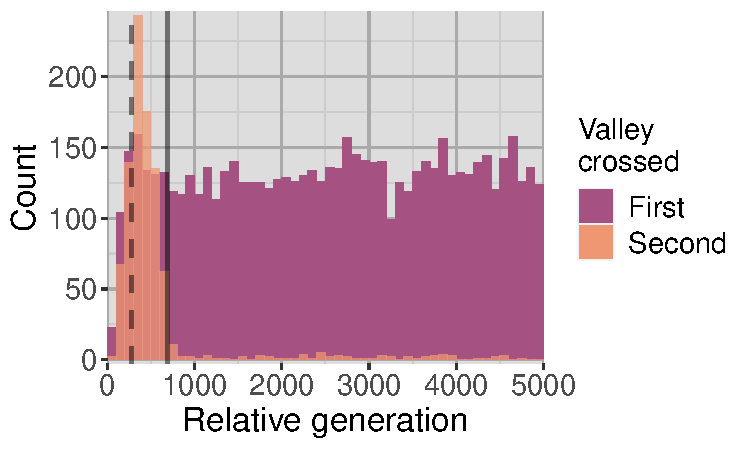
\includegraphics[width=0.45\textwidth]{media/first_two_crosses_overlayed_fair_comparison_with_fixation.pdf}
% \caption{
%     Distribution of the number of updates required to cross valleys in the validation experiment. 
%     Relative updates refer to the number of elapsed generations for the first cross, and the number of generations since the first cross for the second cross. 
%     %The solid and dashed horizontal lines show the expected count of first and second crosses per bar, respectively, for the expected uniform distribution. 
%     The dashed and solid vertical lines show the minimum and maximum fixation times, respectively. 
% }
% \label{fig-crosses-from-scratch}
% \end{center}
% \end{figure}





%Further, we tested the role of disequilibrium in these discoveries by comparing the evolution of populations seeded with eight organisms on $p_{2}$ and the rest on $p_{1}$ (disequilibrium treatment) against whole populations of $p_{2}$ (control). 
%We found that 1,751 of 10,000 disequilibrium replicates crossed the first valley (\localapprox 17.5\%), while only 23 of 10,000 control replicates crossed (\localapprox 0.2\%). 
%This difference is highly significant ($p < 10^{-15}$, Fisher's exact test).
%This further supports the claim that adaptive momentum relies on disequilibrium in the population, and shows that we can start artificially start an adaptive momentum window in this system by creating this disequilibrium. 

\subsection{Empirical benchmarks}

%After confirming that disequilibrium can facilitate valley crosses, we next tested idealized populations to benchmark the effect on valley crossing of two components of this disequilibrium: the position of the leading edge, and the genotypes of the organisms comprising that leading edge.
The empirical benchmark data (Fig. \ref{fig-combined-plots}B) illustrate how the initial state of the population affects the potential to cross valleys.
%In particular the ratio of the population initiated on $p_2$ (mutant type), versus $p_1$ (wild type) and the value of the individuals on the leading edge,
As expected, steps further into the valley increase the probability of crossing, regardless of where the leading edge is. 
On the other hand, the probability of crossing decreases as the ratio of $p_2$ organisms (mutant type) increases relative to $p_1$ organisms (wild type) -- as the selective sweep progresses, fewer opportunities remain for additional mutations to accumulate. 
While the potential to cross varies considerably with the type of organisms in the leading edge, these data clearly show that all conditions describing early sweep conditions (\textit{i.e.}, having a leading edge and a significant ratio of the remaining population on $p_1$) %having any leading edge 
substantially increase the probability of crossing the valley compared to populations that are close to reaching equilibrium on $p_2$. 

%The benchmarks with a leading edge at index 0 see slightly lower rates of crossing, as they only have one organism at the given value while every other point has 8 organ
%We typically ran these benchmarking populations with a leading edge of eight organisms of the same type to remove the possibility of genetic drift immediately destroying the leading edge. 
%This drift accounts for the drop in crosses at index 0, the one instance where the leading edge consisted of only a single organism. 
%Finally, being one step away from crossing the valley ($p_2$ + 5) effectively guarantees a cross, as eight organisms at that value are almost certain to accumulate the one needed mutation unless the selective sweep is almost over. 
%Overall, these data match our expectations. 
We use these results to provide a baseline prediction for the analytic replay experiments. 

% \begin{figure}[h!]
% \begin{center}
% 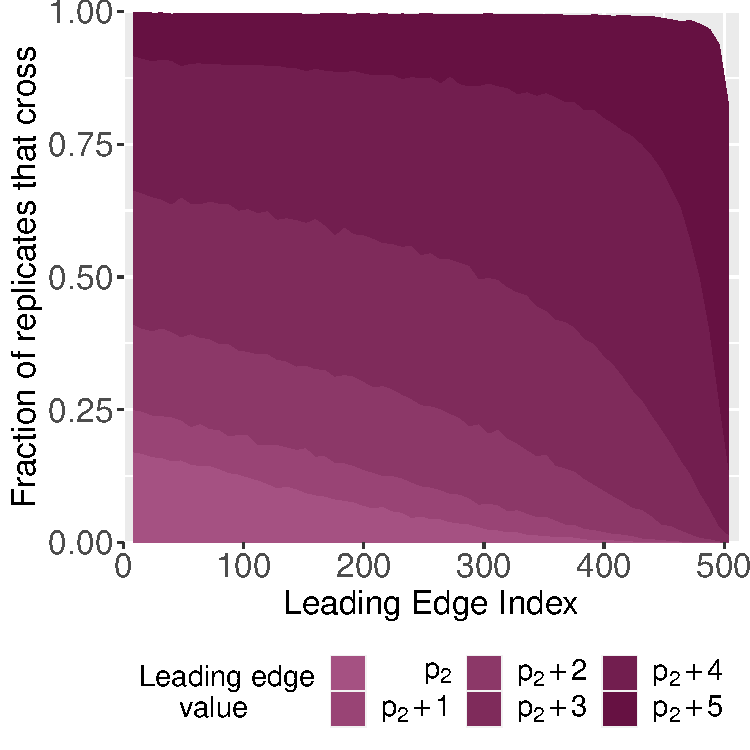
\includegraphics[width=0.45\textwidth]{media/benchmarking_area.pdf}
% \caption{
%     Benchmarking data showing the potential of a leading edge to induce a valley cross, with a range of leading edge values and starting positions. 
%     The leading edge always consists of eight organisms of that value. 
%     Each point represents 10,000 replicates. 
% }
% \label{fig-benchmarking}
% \end{center}
% \end{figure}

\subsection{Analytic replay experiments}
Of our 500 initial replicates to find candidates for replay experiments, four replicates (0.8\%) crossed two valleys in the allotted time, 83 crossed exactly one valley (16.6\%), and the remaining 413 did not cross any valleys (82.6\%). 
%We ran coarse-grained replays for 10 randomly-sampled no-cross replicates, 10 random single-cross replicates, and all four double-cross replicates.
We randomly-sampled 10 no-cross replicates, 10 single-cross replicates, and took all four double-cross replicates to run coarse-grained replays.
%We ran coarse-grained analytic replay experiments for all four replicates that crossed twice and for 10 randomly-sampled replicates of each of the two other categories. 
%For each of these 24 replicates, we replayed at every fourth generation, with 1,000 replicates per time point. 
All plots are available in the supplement \citep{austin_ferguson_2024_11507982}. 

From these coarse-grained replays, we selected one representative replicate from each category to re-run, conducting 10,000 replay trials at \textit{every} time point to give a fine-grained view. 
%We show the replay results in two formats. 
%The first showing the potential of crossing the next valley over time and the second as Muller plots showing the underlying population structure that beget that potentiation. 
For each replayed replicate, we show the potential of crossing the next valley over time, paired with a Muller plot \citep{mullerGeneticAspectsSex1932} of the initial replicate that was replayed. 
Figures \ref{fig-replay-single-cross}, \ref{fig-replay-double-cross}, and \ref{fig-replay-no-cross} show the single-cross, double-cross, and no-cross replicates, respectively. 
%In each plot, the replay results are overlaid atop the benchmarking data, which has been adjusted such that the leading edge index aligns with the actual leading edge at that generation of the population.
In each plot, the replay results are overlaid on an image generated from the benchmark data. 
%To generate the background image, we treat the benchmark data as a lookup function and use the current position of the leading edge of the replay result to look up the potentiation predicted by the benchmark data. 
To generate the background image, we treat the benchmark data as a lookup function.
When we start a replay replicate, we initialize the population using the snapshot from the target generation of the initial replicate. 
These snapshots show that the leading edge does not perfectly advance one position every generation; there are many generations where the leading edge either fails to advance or is pushed back one position by the wild type organisms.
%As we see in our population snapshots, the leading edge does not actually advance one position every generation, the leading often fails to advance, and occasionally the wild-type organisms replicate over the leading edge, pushing it back one step. 
To make this comparison fair, we find the leading edge in that particular snapshot and then look up the corresponding expectation values from the benchmark data. 
%Thus, the background image shows in ``real time'' potentiation of the replay at each generation.
This adjustment ensures that we are comparing against the correct benchmark data regardless of the motion of the leading edge. 
%Thus, the background image adjusts 

Overall, the potentiation observed in all three replicates closely match the benchmark expectations. 
The potentiation occasionally increases or decreases suddenly; tracing these changes to the Muller plots typically shows that these events correlate to the gain or loss of a mutation at (or near) the leading edge at that time. 
For example, the two temporary peaks in potential in Figure \ref{fig-replay-single-cross}, at roughly generations 250 and 375, can be directly traced to the leading edge temporarily dipping to $p_{2} + 4$.
%When the leading edge mutates further into the fitness valley, the potentiation increases dramatically. 
%Each of the three replicates 
The potentiation at any particular step in the valley decreases over time, as the selective sweep progresses and the adaptive momentum window closes.
Figure \ref{fig-replay-no-cross} shows that, while the replicate had substantial potentiation at times (briefly above 50\%), it failed to capitalize before the window closed. 
This failure was exacerbated by two leading mutations from $p_{2} + 3$ to $p_{2} + 2$, the second of which dropped the potential from over 25\% to under 10\%, after which the population never recovers. 
% It should be noted that the dramatic increases or decreases in potentiation can be mapped cleanly onto the Muller plots showing the state of the population. 
% For example, in Figure \ref{fig-replay-single-cross} potentiation temporarily increases dramatically (from \localapprox 60\% to \localapprox 90\%) twice, once around update 250 and again around update 350. 
% In both cases, the potentiation then drops to previous levels shortly after. 
% Mapping this points onto the Muller plot, we see that, in both cases, the leading edge drifted down an additional step into the valley (to $p_{1} + 4$) before quickly drifting back to the previous step. 
% These drops in potentiation are particularly dramatic in the no-cross replicate of Figure \ref{fig-replay-no-cross}, where a late drift backward reduces the potential to cross from over 25\% to under 10\%, from which the population never recovers. 

All three replicates show periods of potentiation higher than what our benchmark data would predict given their leading edge genomic value. 
The benchmarking data modeled a leading edge of eight organisms, but the Muller plots show that the leading edge grows and shrinks over time. 
The Muller plots show that underprediction is generally associated with either an expanded leading edge or an excess of individuals with lower fitness behind the leading edge. 
We hypothesize that these underpredictions are generally observed in deeper steps into the valley because of the historical contingency required to reach that point (\textit{i.e.}, to reach $p_{2} + 5$ the leading edge must have passed through $p_{2} + 4$, which may still exist behind the leading edge).
%While all organisms behind the leading edge are experiencing purifying selection, this purification takes time, and a cluster of mutated organisms can persist behind the leading edge. 
%Our benchmark expectations are particularly accurate for early steps into the valley; even if a large cluster of organisms exists behind the leading edge, they are still unlikely to accumulate the needed mutations to cross the valley before being purified. 
%In contrast, when the leading edge is only a mutation or two away from crossing, even a few organisms trailing the leading edge can be enough to cross the valley. 
%If a sizable section of the population is only two or three mutations from crossing the valley, the size of that section may buffer the organisms from purifying selection long enough for some organisms to genetically drift to the next peak. 
%This is supported by the replays almost perfectly aligning with the expectation in the first few steps into the valley, where the mutation rate cannot outpace the rate of purifying selection, while the empirical potentiation is often above the expectation in the last few steps of the valley. 
%This was not explicitly modeled in the benchmarking data, possibly causing this difference. 
%while replays see leading edges that are much larger or smaller, causing some variation from the expectation.
%Further, our benchmarks are based \textit{only} on the leading edge, and thus our hypothesis is that this higher-than-expected potentiation results from the evolutionary potential of non-leading edge organisms. 

\begin{figure}[h!]
\begin{center}
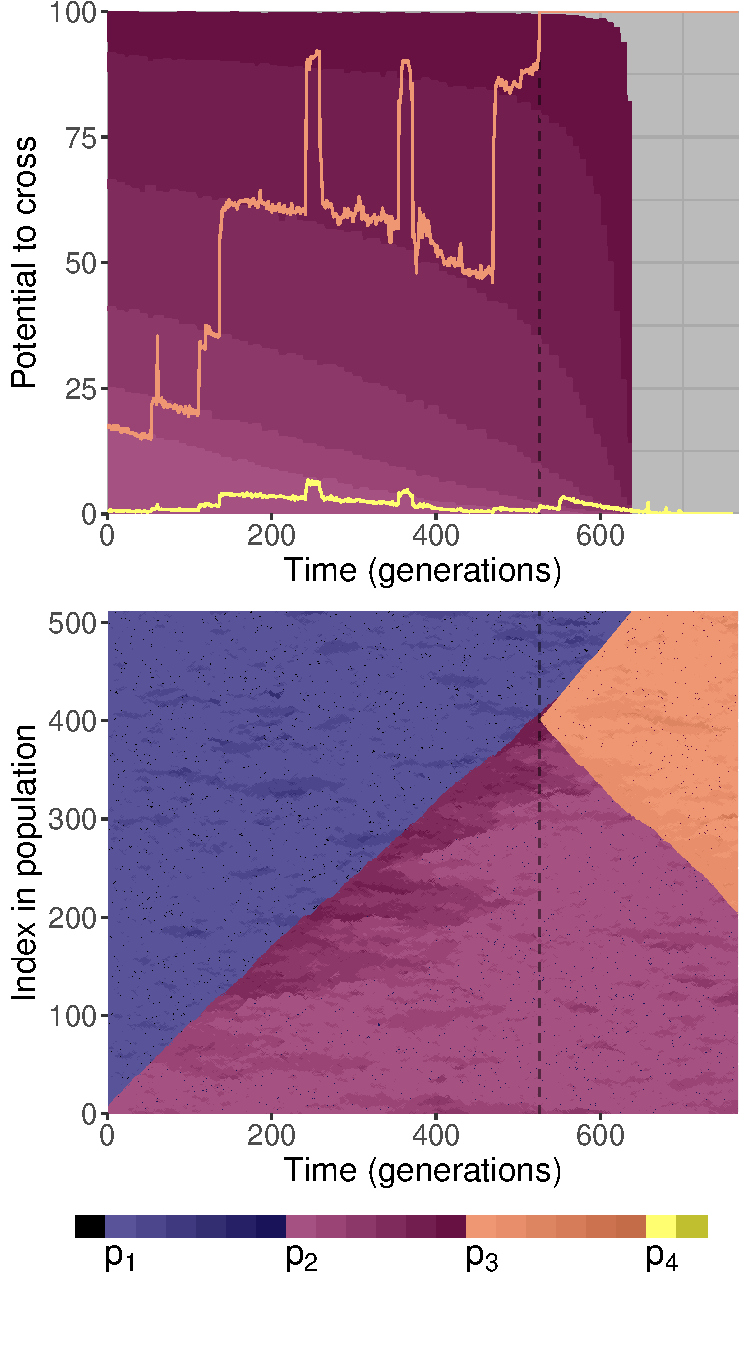
\includegraphics[width=0.6\textwidth]{05_adaptive_momentum/media/reps/400/script_06__plot_05__combined_plot_area_palette.pdf}
\caption{
    Top plot: Analytic replay data for a representative replicate that crossed one valley during a momentum window, overlayed on baseline data. 
    Lines show the probability of crossing both the first valley  (orange line; initially-higher) and the second valley (yellow line; initially-lower). 
    The background shows the expected potential to cross (as shown in Fig. \ref{fig-combined-plots}B); data here are shifted to align with the realized leading edge position. 
    %Each update was replayed 10,000 times. 
    Bottom plot: A Muller plot of all organisms in the original 1D population over time. 
    Dark colors show descent into valleys, with hue identifying the valley being crossed. 
    In both plots, vertical dashed lines show initial valley crosses.
    Colors in the legend apply to all plots. 
}
\label{fig-replay-single-cross}
\end{center}
\end{figure}

\begin{figure}[h!]
\begin{center}
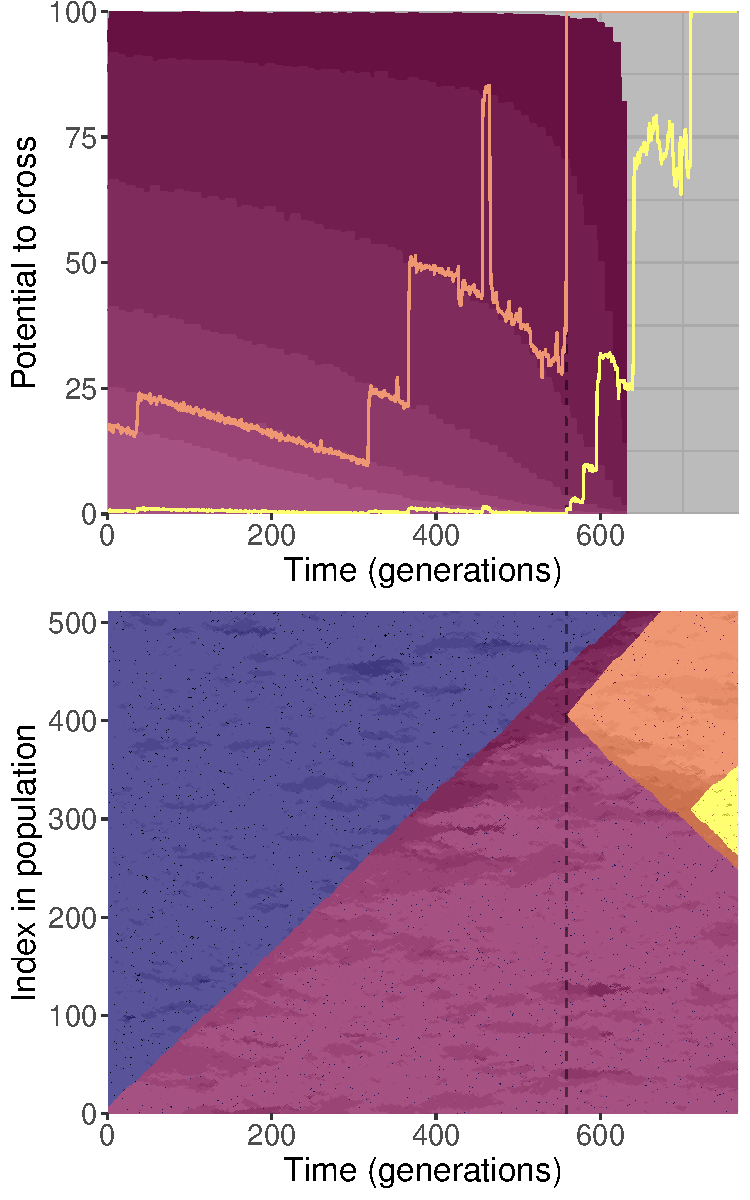
\includegraphics[width=0.6\textwidth]{05_adaptive_momentum/media/reps/263/script_06__plot_03__combined_plot_area.pdf}
\caption{
    The analytic replay data for a representative replicate that crossed two valleys during a momentum window. 
    See Figure \ref{fig-replay-single-cross} for details and legend. 
}
\label{fig-replay-double-cross}
\end{center}
\end{figure}

\begin{figure}[h!]
\begin{center}
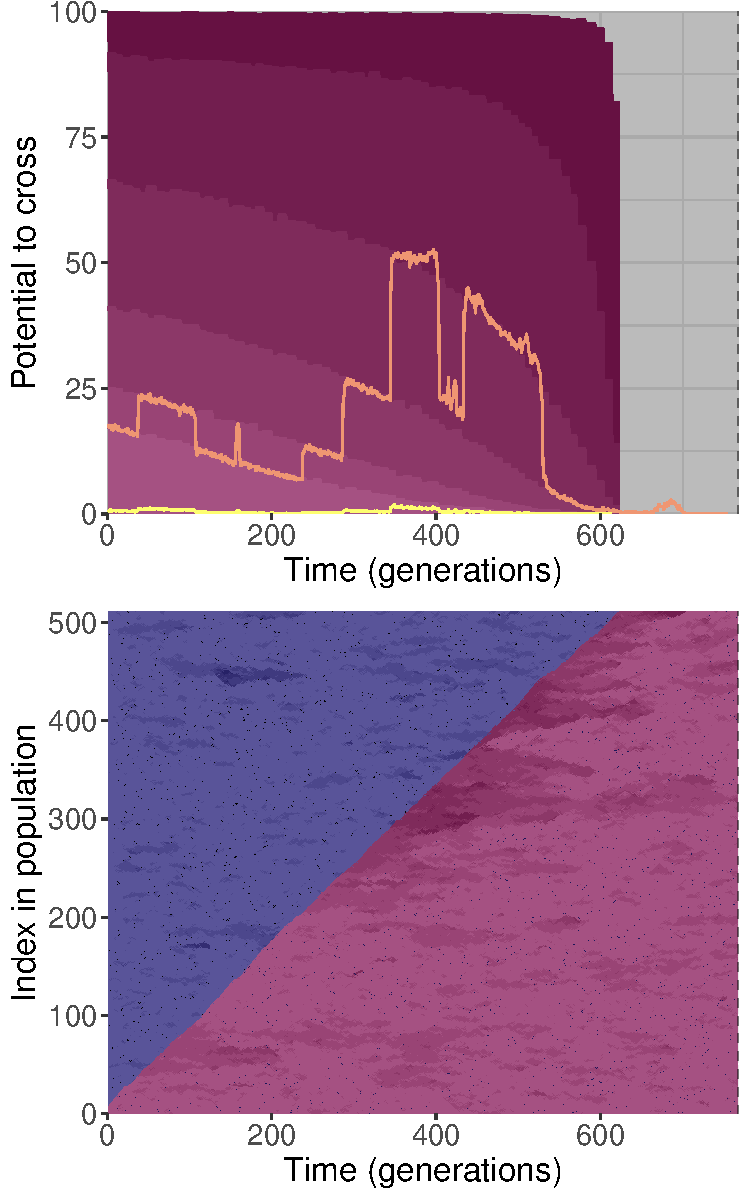
\includegraphics[width=0.6\textwidth]{05_adaptive_momentum/media/reps/339/script_06__plot_03__combined_plot_area.pdf}
\caption{
    The analytic replay data for a representative replicate that failed to cross a valley during a momentum window.
    See Figure \ref{fig-replay-single-cross} for details and legend.
}
\label{fig-replay-no-cross}
\end{center}
\end{figure}

For comparison, we also ran 10,000 replicates that started at equilibrium (\textit{i.e.}, not in a momentum window).
Of those, we replayed the one replicate that crossed twice, 10 randomly sampled replicates from 19 that crossed once, and 10 random replicates from the 9,980 that failed to cross. 
Figure \ref{fig-replay-no-window} shows the replicate that crossed twice. 
The first crossing in this replicate occurred quite early, crossing the valley on generation 168. 
However, the potential before crossing is similar to all first-cross replicates: while the potential in an adaptive momentum window starts at \localapprox 17\%, the potential for replicates outside momentum windows starts at \localapprox 0.2\%. 
This low potential continues for the first 143 generations, followed by 16 generations with an average potential of \localapprox 1.8\%, four generations between 15\% and 20\%, and then the cross. 
%This pure chance, ``all or nothing'' potentiation is not unique to this replicate, as we see in the histograms of potential shown in Figure \ref{fig-histograms}.
This pure chance, ``all or nothing'' potentiation is not unique to this replicate; the same dynamic can be seen in the ten other successful replicates we analyzed \citep{austin_ferguson_2024_11507982}.
% Figure \ref{fig-replay-no-window} shows the potential for the first and second valley crossing. 
% The potential for the first valley crossing remains very low ($<$0.4\%) until it increased to 100\% in less than 20 generations. 
% This increase is not linear, however, as there is an initial increase and then a drop in potentiation, likely corresponding to the flux in $p_{2} + 5$ organisms in the population. 
% The discovery of $p_{3}$ starts a momentum window, and the potential of the second cross then looks like the potential in previous results (although limited by the lack of remaining time), and is higher than the potential of the first window was for the first \localapprox 580 generations.


\begin{figure}[h!]
\begin{center}
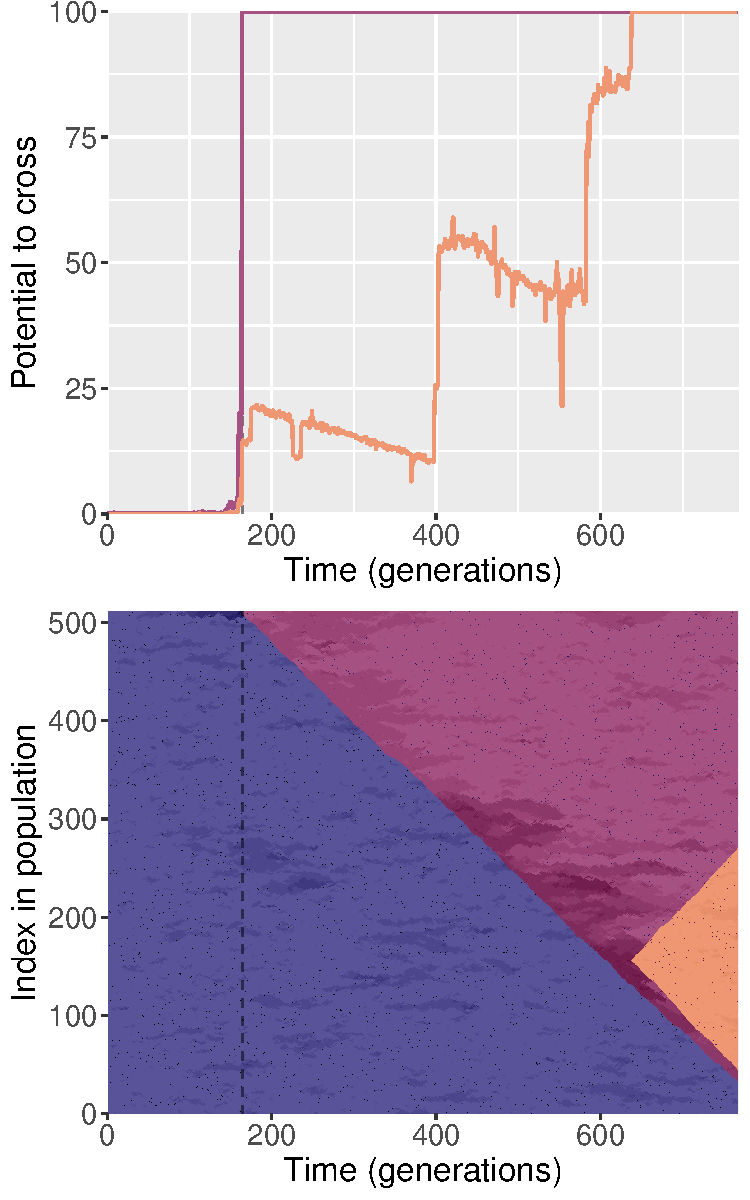
\includegraphics[width=0.6\textwidth]{05_adaptive_momentum/media/reps/no_am_two_cross/script_06__plot_02__combined_plot.pdf}
\caption{
    \textbf{Top plot}: The analytic replay data for the sole replicate that did \textit{not} start in a momentum window, but still managed to cross a valley, and indeed crossed twice. 
    The red line shows the potential to cross the first valley, while the orange line shows the potential to cross the second valley, exhibiting the hallmarks of adaptive momentum due to the first cross. 
    \textbf{Bottom plot}: a Muller plot of the original population, like in Figure \ref{fig-replay-single-cross}.
}
\label{fig-replay-no-window}
\end{center}
\end{figure}

Finally, we also show the potentiation of crossing the second valley, which in some cases is realized (Figs. \ref{fig-replay-double-cross} and \ref{fig-replay-no-window}), and other times is not (Figs. \ref{fig-replay-single-cross} and \ref{fig-replay-no-cross}).
As potentiation is probabilistic in nature, the potential to cross the second valley is the probability of crossing the first valley from the current state of the population times the probability of crossing a second valley from a na\"ive starting position (\textit{i.e.}, the elevated potentiation of a population at the beginning of a sweep). 
We see this dynamic early in the replays -- increases in first-cross potential are reflected, at smaller scales, in second-cross potential,
%Once the first valley is crossed, the potential to cross the second valley can increase dramatically. 
%Indeed, we see sizable increases in second-cross potential 
with a much larger increase upon successful crossing of the first valley in Figures \ref{fig-replay-single-cross} and \ref{fig-replay-double-cross}. %, \ref{fig-replay-no-window}, and . 
This result is consistent with the adaptive momentum framework, which posits that the discovery of a new peak will initiate a new adaptive momentum window. 
Strikingly, this same dynamic holds true for Figure \ref{fig-replay-no-window} -- while the replicate did not start in a momentum window, the first cross creates a window which increases the potential of the second cross.

\subsection{Shuffled population experiments}

To test the importance of population structure for potentiation, we repeated the benchmarking and replay experiments with shuffled populations. 
In both cases, we kept the experiments identical except for an additional shuffle step: before starting a replicate, we shuffled the order of organisms in the population and then proceeded with evolution as normal. 
%We replayed the evolution of 10 randomly-sampled single-cross replicates, and 

The shuffled benchmark data in Figure \ref{fig-combined-plots}C shows that only populations with a leading edge of $p_{2} + 5$ are able to maintain greater than a 10\% chance to cross if the leading edge has swept more than half the population.
Two differences can decrease crossing potential: 
1) multiple leading edges can form, allowing faster fixation and 
2) the eight leading-edge organisms are more likely to encounter higher-fitness mutant-type organisms and thus be purified faster.
%When the benchmark populations are shuffled, fixation occurs more rapidly and thus the potential to cross falls quickly.  

A representative sample from the single-cross replicates is shown in Figure \ref{fig-replay-shuffle}. 
The replay data indicate that potential to cross remains relatively low, never reaching a 20\% chance, until a critical mass of nearly-crossed organisms skyrockets the potential from 9.2\% to 100\%. 
The earlier spikes in potentiation always correspond to the appearance of a single organism that is one step away from crossing the valley, which was then lost in the original population.
These trends are consistent across all 10 replicates that were replayed \citep{austin_ferguson_2024_11507982}. 

\begin{figure}[h!]
\begin{center}
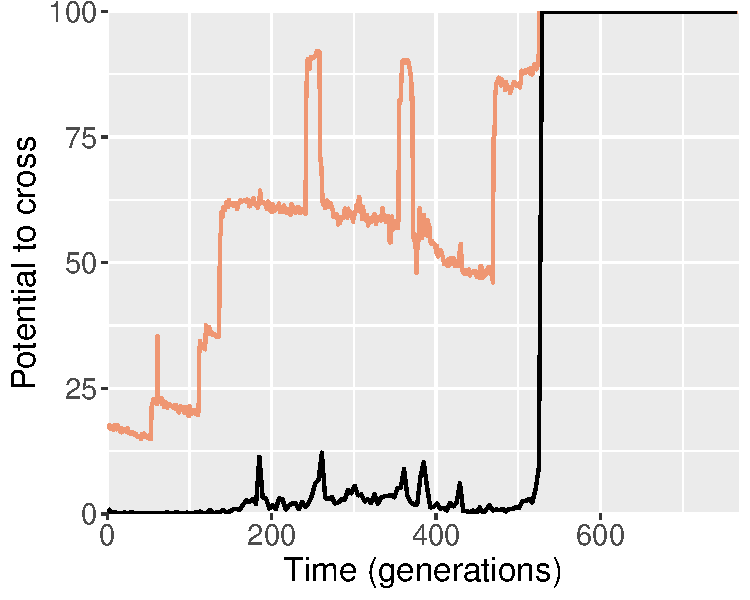
\includegraphics[width=0.6\textwidth]{05_adaptive_momentum/media/reps/400/script_07__plot_01__selected_replays_with_shuffled_replays_no_bg.pdf}
\caption{
    The black line (bottom) shows the potential for a shuffled population to cross a valley. 
    The orange line (top) shows the standard potential for the population to cross (same data as Fig. \ref{fig-replay-single-cross}). 
    The shuffled line consists of 1,000 samples every 4 generations. 
    %Background shading shows the expected potential to cross when an idealized leading edge population is shuffled (a shuffled version of Figure \ref{fig-benchmarking}). 
}
\label{fig-replay-shuffle}
\end{center}
\end{figure}

% \begin{figure}[h!]
% \begin{center}
% 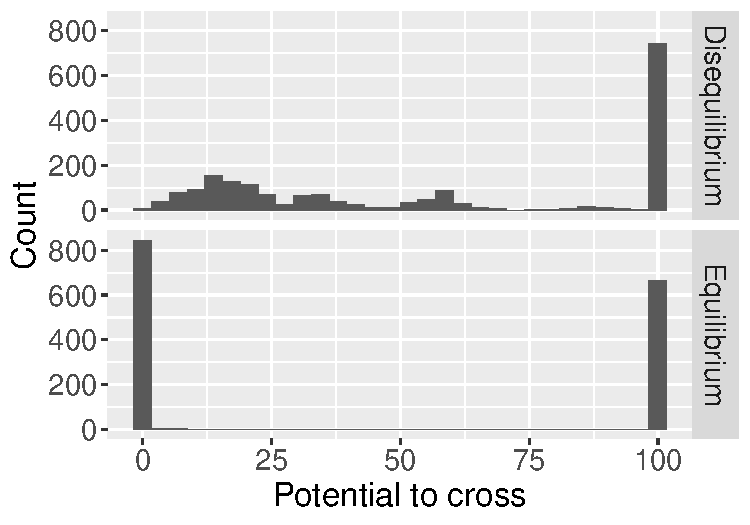
\includegraphics[width=0.45\textwidth]{media/combined_potentiation_histograms.pdf}
% \caption{
%     Histogram of potentiation values in replicates in a momentum window (disequilibrium, top) and outside a window (equilibrium, bottom).
% }
% \label{fig-histograms}
% \end{center}
% \end{figure}









% \section{Results}
% %Below we describe the results in the same order the experiments were described, first validating the adaptive momentum effect, then moving onto benchmarking and replay experiment results.  

% \begin{figure*}[h!]
% \begin{center}
% 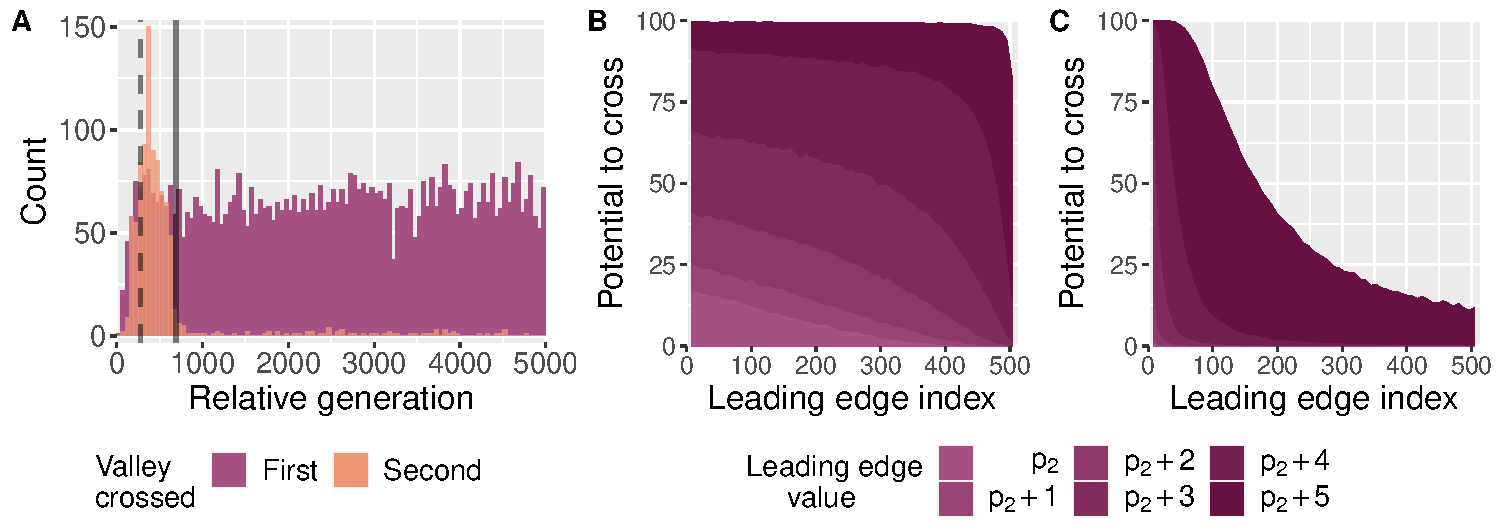
\includegraphics[width=\textwidth]{05_adaptive_momentum/media/combined_plots_full_split.pdf}
% \caption{
%     \textbf{(A)}
%     Distribution of the number of generations required to cross valleys in the validation experiment. 
%     Relative generations refer to the number of elapsed generations for the first cross, and the number of generations since the first cross for the second cross. 
%     %The solid and dashed horizontal lines show the expected count of first and second crosses per bar, respectively, for the expected uniform distribution. 
%     The dashed and solid vertical lines show the minimum and maximum fixation times, respectively. 
%     \textbf{(B)} 
%     Benchmarking data showing the potential of a leading edge to induce a valley cross, with a range of leading edge values and starting positions (see Figure \ref{fig-experiment2}). 
%     Each point represents 10,000 replicates.
%     \textbf{(C)}
%     Shuffled benchmarking data. Each replicate is shuffled prior to evolution, otherwise identical to center plot.
% }
% \label{fig-combined-plots}
% \end{center}
% \end{figure*}

% \subsection{Validation of adaptive momentum effect}

% First, we measured the time it took for replicates starting from a full population of $p_{2}$ to cross valleys.
% Figure \ref{fig-combined-plots}A
% shows the timing distributions of populations that crossed the first valley over the first 5,000 generations (red) as well as the timing distributions of second crossings that occur within 5,000 generations of a first (orange). 
% We see that the time of first crossing appear uniformly distributed across the 5,000 generations, while the second crosses are strongly biased toward shorter time periods. 
% Indeed, of 500,000 replicates, 6,485 crossed the first valley within 5,000 generations (\localapprox 1.3\%) with a mean cross time of \localapprox 2,569 generations and a median of 2,602 generations. 
% Based on these values, we would expect roughly 84 replicates to cross twice ($6,485 \times 1.3\%$, or 0.0169\% of all 500,000 replicates), but instead we see 902 replicates (\localapprox 0.18\%) cross the second valley, showing a much higher rate of second crossing than expected if the probabilities of first and second crossing were equal.
% In addition to a higher than expected rate of crossing, the mean cross time between first and second crossings is \localapprox 579 generations and the median cross time is 401 generations, substantially lower than the first crossing times. 
% Finally, when we consider only those second crossing times that occurred more than 1000 generations after a first crossing, we find that the rate of these second crossings is similar to the first crossing rate (\localapprox 1.23\%).
% These results comport with the framework of adaptive momentum. 
% They show that an initial beneficial discovery can quickly lead to additional discoveries (during the fixation period), but if the second discovery does not happen before equilibrium is reestablished, the rate of valley crossing is better predicted by the first valley crossing times. 


% % Indeed, of 500,000 replicates, 12,793 crossed at least once (\localapprox 2.6\%) with a mean cross time of \localapprox 4,995 generations and a median of 4,951 generations. 
% % We would expect that only 338 replicates to cross twice (2.6\% squared), but instead we see 1,734 replicates cross at least two valleys (\localapprox 0.35\% of total, or \localapprox 13.6\% of those that crossed once). 
% % For the second crossings, we see a mean cross time of 646 generations and a median cross time of 396 generations. 
% % Indeed, while not shown in Figure \ref{fig-crosses-from-scratch}, we see 200 replicates cross at least three valleys, 26 replicates cross at least four valleys, and six replicates cross five valleys; of these higher-order crossings, the median time to cross was always less than 420 generations. 
% % These findings, where an initial beneficial discovery can quickly lead to additional discoveries, supports the initial adaptive momentum theory. 

% % \begin{figure}[h!]
% % \begin{center}
% % 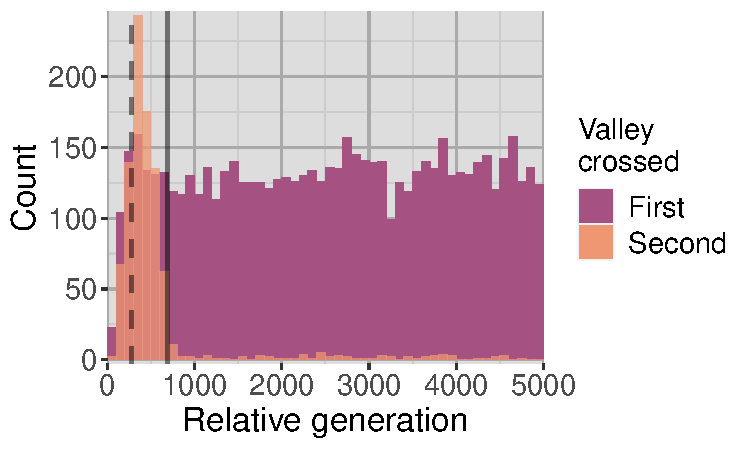
\includegraphics[width=0.45\textwidth]{media/first_two_crosses_overlayed_fair_comparison_with_fixation.pdf}
% % \caption{
% %     Distribution of the number of updates required to cross valleys in the validation experiment. 
% %     Relative updates refer to the number of elapsed generations for the first cross, and the number of generations since the first cross for the second cross. 
% %     %The solid and dashed horizontal lines show the expected count of first and second crosses per bar, respectively, for the expected uniform distribution. 
% %     The dashed and solid vertical lines show the minimum and maximum fixation times, respectively. 
% % }
% % \label{fig-crosses-from-scratch}
% % \end{center}
% % \end{figure}





% %Further, we tested the role of disequilibrium in these discoveries by comparing the evolution of populations seeded with eight organisms on $p_{2}$ and the rest on $p_{1}$ (disequilibrium treatment) against whole populations of $p_{2}$ (control). 
% %We found that 1,751 of 10,000 disequilibrium replicates crossed the first valley (\localapprox 17.5\%), while only 23 of 10,000 control replicates crossed (\localapprox 0.2\%). 
% %This difference is highly significant ($p < 10^{-15}$, Fisher's exact test).
% %This further supports the claim that adaptive momentum relies on disequilibrium in the population, and shows that we can start artificially start an adaptive momentum window in this system by creating this disequilibrium. 

% \subsection{Empirical benchmarks}

% %After confirming that disequilibrium can facilitate valley crosses, we next tested idealized populations to benchmark the effect on valley crossing of two components of this disequilibrium: the position of the leading edge, and the genotypes of the organisms comprising that leading edge.
% The empirical benchmark data (Figure \ref{fig-combined-plots}B) illustrate how the initial state of the population affects the potential to cross valleys.
% %In particular the ratio of the population initiated on $p_2$ (mutant type), versus $p_1$ (wild type) and the value of the individuals on the leading edge,
% As expected, steps further into the valley increase the probability of crossing, regardless of where the leading edge is. 
% On the other hand, the probability of crossing decreases as the ratio of $p_2$ organisms (mutant type) increases relative to $p_1$ organisms (wild type) -- as the selective sweep progresses there are fewer opportunities remaining for additional mutations to accumulate. 
% While the potential to cross varies considerably with the type of organisms in the leading edge, these data clearly show that all conditions describing early sweep conditions (i.e., having leading edge and a significant ratio of the remaining population on $p_1$) %having any leading edge 
% substantially increase the probability of crossing the valley compared to populations that are close to reaching equilibrium on $p_2$. 

% %The benchmarks with a leading edge at index 0 see slightly lower rates of crossing, as they only have one organism at the given value while every other point has 8 organ
% %We typically ran these benchmarking populations with a leading edge of eight organisms of the same type to remove the possibility of genetic drift immediately destroying the leading edge. 
% %This drift accounts for the drop in crosses at index 0, the one instance where the leading edge consisted of only a single organism. 
% %Finally, being one step away from crossing the valley ($p_2$ + 5) effectively guarantees a cross, as eight organisms at that value are almost certain to accumulate the one needed mutation unless the selective sweep is almost over. 
% %Overall, these data match our expectations. 
% We use these results to provide a baseline prediction for the analytic replay experiments. 

% % \begin{figure}[h!]
% % \begin{center}
% % 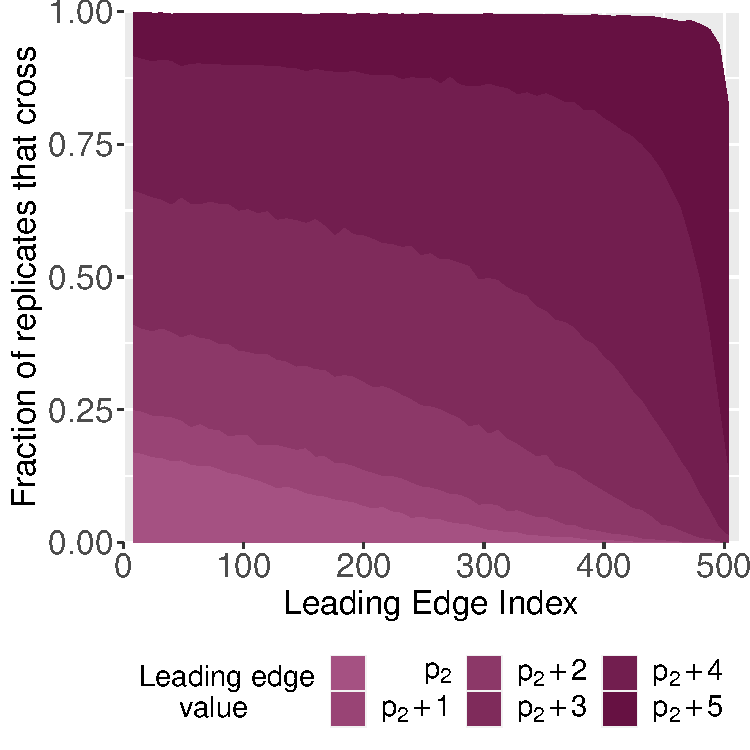
\includegraphics[width=0.45\textwidth]{media/benchmarking_area.pdf}
% % \caption{
% %     Benchmarking data showing the potential of a leading edge to induce a valley cross, with a range of leading edge values and starting positions. 
% %     The leading edge always consists of eight organisms of that value. 
% %     Each point represents 10,000 replicates. 
% % }
% % \label{fig-benchmarking}
% % \end{center}
% % \end{figure}

% \subsection{Analytic replay experiments}
% Of our 500 initial replicates to find candidates for replay experiments, four replicates (0.8\%) crossed two valleys in the allotted time, 83 crossed exactly one valley (16.6\%), and the remaining 413 did not cross any valleys (82.6\%). 
% We ran coarse-grained replays for 10 randomly-sampled no-cross replicates, 10 random single-cross replicates, and all four double-cross replicates.
% %We ran coarse-grained analytic replay experiments for all four replicates that crossed twice and for 10 randomly-sampled replicates of each of the two other categories. 
% %For each of these 24 replicates, we replayed at every fourth generation, with 1,000 replicates per time point. 
% All plots are available in the supplement \citep{austin_ferguson_2024_11507982}. 

% From these coarse-grained replays, we selected one representative replicate from each category. 
% We re-ran these representative replicates, conducting 10,000 replay trials at \textit{every} time point to give a fine-grained view. 
% %We show the replay results in two formats. 
% %The first showing the potential of crossing the next valley over time and the second as Muller plots showing the underlying population structure that beget that potentiation. 
% For each replayed replicate, we show the potential of crossing the next valley over time, paired with a Muller plot \citep{mullerGeneticAspectsSex1932} of the initial replicate that was replayed. 
% Figures \ref{fig-replay-single-cross}, \ref{fig-replay-double-cross}, and \ref{fig-replay-no-cross} show the single-cross, double-cross, and no-cross replicates, respectively. 
% %In each plot, the replay results are overlaid atop the benchmarking data, which has been adjusted such that the leading edge index aligns with the actual leading edge at that generation of the population.
% In each plot, the replay results are overlaid atop an image generated from the benchmark data. 
% %To generate the background image, we treat the benchmark data as a lookup function and use the current position of the leading edge of the replay result to look up the potentiation predicted by the benchmark data. 
% To generate the background image, we treat the benchmark data as a lookup function. 
% When we start a replay replicate, we initialize the population using the snapshot from a particular generation of the initial replicate. 
% These snapshots show that the leading edge does not perfectly advance one position every generation; there are many generations where the leading edge either fails to advance or is pushed back one position by the wild type organisms.
% %As we see in our population snapshots, the leading edge does not actually advance one position every generation, the leading often fails to advance, and occasionally the wild-type organisms replicate over the leading edge, pushing it back one step. 
% To make this comparison fair, we find the leading edge in that particular snapshot and then look up the corresponding expectation values from the benchmark data. 
% %Thus, the background image shows in ``real time'' potentiation of the replay at each generation.
% This adjustment ensures that we are comparing against the correct benchmark data regardless of the motion of the leading edge. 
% %Thus, the background image adjusts 

% Overall, the potentiation observed in all three replicates closely match the benchmark expectations. 
% The potentiation occasionally increases or decreases suddenly; tracing these changes to the Muller plots typically shows that these events correlate to the gain or loss of a mutation at (or near) the leading edge at that time. 
% For example, the two temporary peaks in potential in Figure \ref{fig-replay-single-cross}, at roughly generations 250 and 375, can be directly traced to the leading edge temporarily dipping to $p_{2} + 4$.
% %When the leading edge mutates further into the fitness valley, the potentiation increases dramatically. 
% %Each of the three replicates 
% The potentiation at any particular step in the valley decreases over time, as the selective sweep progresses and the adaptive momentum window closes.
% Figure \ref{fig-replay-no-cross} clearly shows that, while the replicate had substantial potentiation at times (briefly above 50\%), it failed to capitalize before the window closed. 
% This failure was exacerbated by two leading mutations from $p_{2} + 3$ to $p_{2} + 2$, the second of which dropped the potential from over 25\% to under 10\%, after which the population never recovers. 
% % It should be noted that the dramatic increases or decreases in potentiation can be mapped cleanly onto the Muller plots showing the state of the population. 
% % For example, in Figure \ref{fig-replay-single-cross} potentiation temporarily increases dramatically (from \localapprox 60\% to \localapprox 90\%) twice, once around update 250 and again around update 350. 
% % In both cases, the potentiation then drops to previous levels shortly after. 
% % Mapping this points onto the Muller plot, we see that, in both cases, the leading edge drifted down an additional step into the valley (to $p_{1} + 4$) before quickly drifting back to the previous step. 
% % These drops in potentiation are particularly dramatic in the no-cross replicate of Figure \ref{fig-replay-no-cross}, where a late drift backward reduces the potential to cross from over 25\% to under 10\%, from which the population never recovers. 

% All three replicates show periods of potentiation higher than what our benchmark data would predict given their leading edge genomic value. 
% The benchmarking data modeled a leading edge of eight organisms, but the Muller plots show that the leading edge grows and shrinks over time. 
% The Muller plots show that overprediction is generally associated with either an expanded leading edge or an excess of individuals with lower fitness behind the leading edge. 
% We hypothesized that these overpredictions are generally observed in deeper steps into the valley because of the historical contingency required to reach that point (i.e., to reach $p_{2} + 5$ the leading edge must have passed through $p_{2} + 4$, which may still exist behind the leading edge).
% %While all organisms behind the leading edge are experiencing purifying selection, this purification takes time, and a cluster of mutated organisms can persist behind the leading edge. 
% %Our benchmark expectations are particularly accurate for early steps into the valley; even if a large cluster of organisms exists behind the leading edge, they are still unlikely to accumulate the needed mutations to cross the valley before being purified. 
% %In contrast, when the leading edge is only a mutation or two away from crossing, even a few organisms trailing the leading edge can be enough to cross the valley. 
% %If a sizable section of the population is only two or three mutations from crossing the valley, the size of that section may buffer the organisms from purifying selection long enough for some organisms to genetically drift to the next peak. 
% %This is supported by the replays almost perfectly aligning with the expectation in the first few steps into the valley, where the mutation rate cannot outpace the rate of purifying selection, while the empirical potentiation is often above the expectation in the last few steps of the valley. 
% %This was not explicitly modeled in the benchmarking data, possibly causing this difference. 
% %while replays see leading edges that are much larger or smaller, causing some variation from the expectation.
% %Further, our benchmarks are based \textit{only} on the leading edge, and thus our hypothesis is that this higher-than-expected potentiation results from the evolutionary potential of non-leading edge organisms. 

% \begin{figure}[h!]
% \begin{center}
% 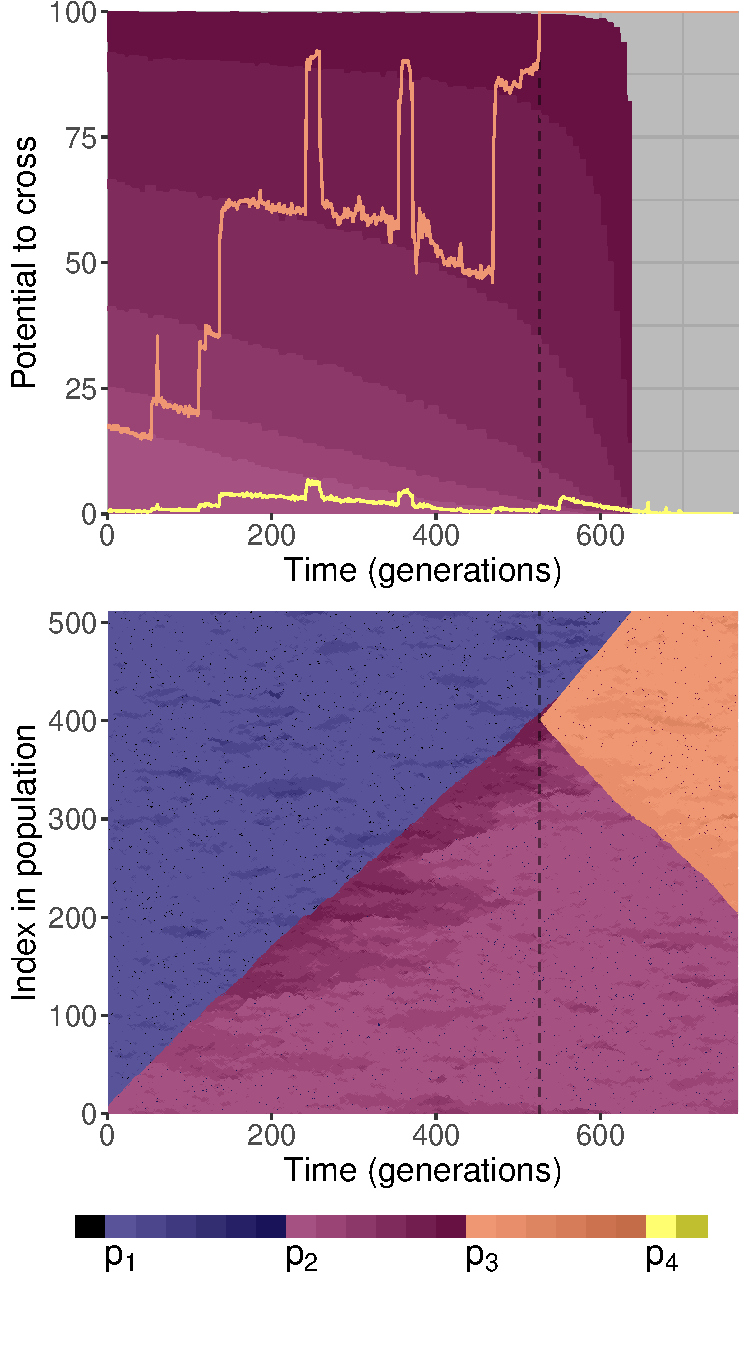
\includegraphics[width=0.6\textwidth]{05_adaptive_momentum/media/reps/400/script_06__plot_05__combined_plot_area_palette.pdf}
% \caption{
%     \textbf{Top plot}: The analytic replay data for a representative replicate that crossed one valley during a momentum window. 
%     The two lines show the probability of crossing valleys, with the initially-higher (orange) line showing the first valley cross and the initially-lower (yellow) line showing the second valley cross. 
%     The background shading shows the expected potential to cross (as shown in Figure \ref{fig-combined-plots}B), adjusted by the actual leading edge of the population. 
%     Each update was replayed 10,000 times. 
%     \textbf{Bottom plot}: A Muller plot of the original population over time. 
%     Dark colors show descent into a valley, with hue identifying the valley being crossed. 
%     In both plots, vertical lines show valley crosses.
%     Colors in the legend apply to all plots. 
% }
% \label{fig-replay-single-cross}
% \end{center}
% \end{figure}

% \begin{figure}[h!]
% \begin{center}
% 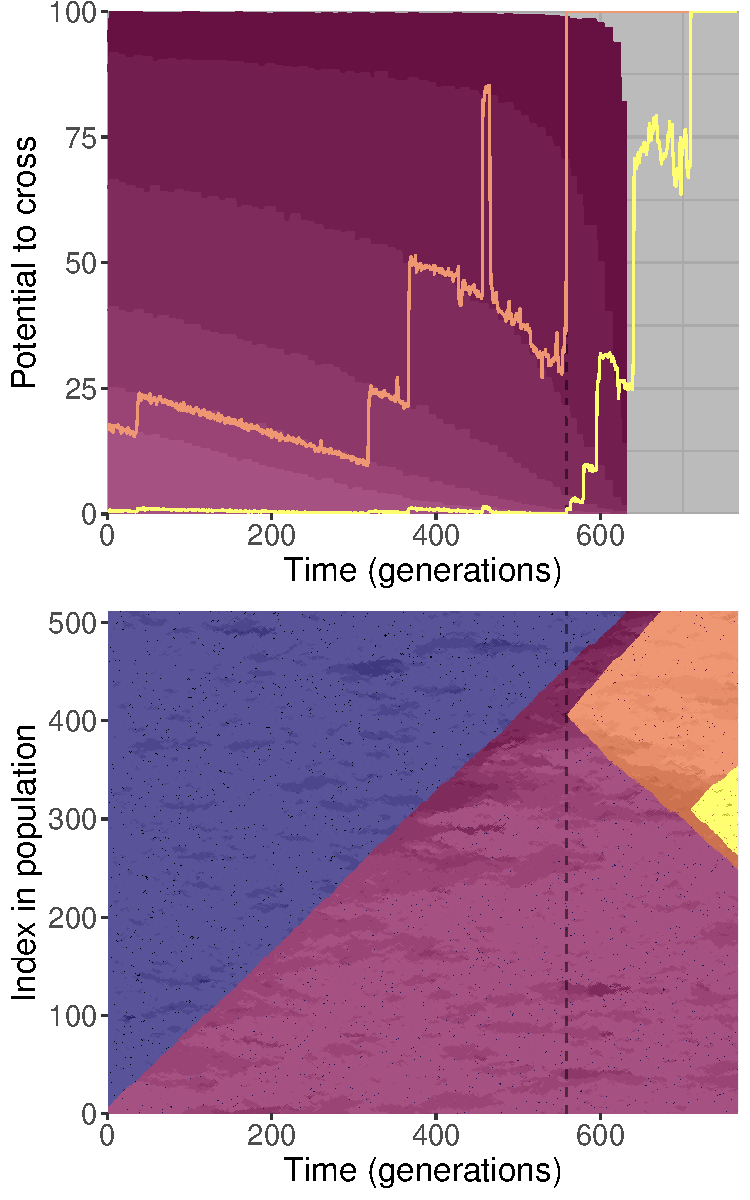
\includegraphics[width=0.6\textwidth]{05_adaptive_momentum/media/reps/263/script_06__plot_03__combined_plot_area.pdf}
% \caption{
%     The analytic replay data for a representative replicate that crossed two valleys during a momentum window. 
%     See Figure \ref{fig-replay-single-cross} for details and legend. 
% }
% \label{fig-replay-double-cross}
% \end{center}
% \end{figure}

% \begin{figure}[h!]
% \begin{center}
% 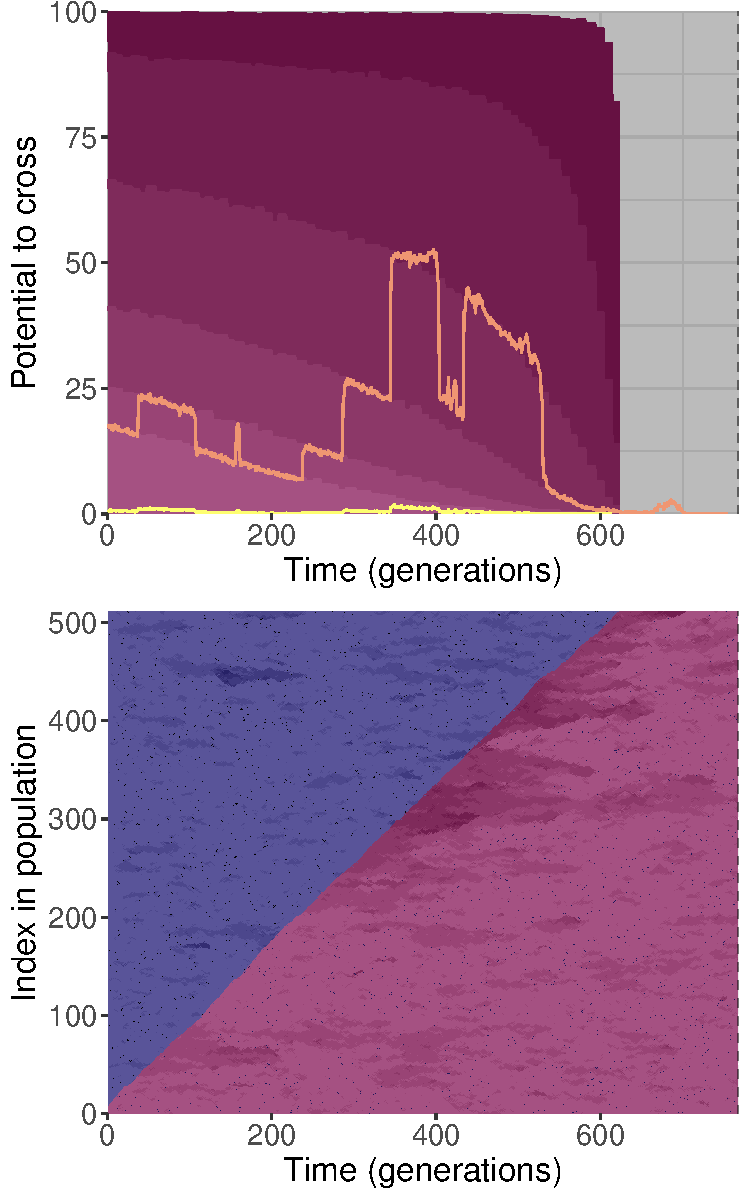
\includegraphics[width=0.6\textwidth]{05_adaptive_momentum/media/reps/339/script_06__plot_03__combined_plot_area.pdf}
% \caption{
%     The analytic replay data for a representative replicate that failed to cross a valley during a momentum window.
%     See Figure \ref{fig-replay-single-cross} for details and legend.
% }
% \label{fig-replay-no-cross}
% \end{center}
% \end{figure}

% For comparison, we also replayed replicates that did not start in a momentum window. 
% We replayed the one replicate in 10,000 that crossed twice, 10 randomly sampled replicates that crossed once, and 10 random replicates that failed to cross. 
% Figure \ref{fig-replay-no-window} shows the replicate that crossed twice. 
% The first crossing in this replicate occurred quite early, crossing the valley on generation 168. 
% However, the potential before crossing is similar to all first-cross replicates: while the potential in an adaptive momentum window starts at \localapprox 17\%, the potential for replicates outside momentum windows starts at \localapprox 0.2\%. 
% This low potential continues for the first 143 generations, followed by 16 generations with an average potential of \localapprox 1.8\%, four generations between 15\% and 20\%, and then the cross. 
% %This pure chance, ``all or nothing'' potentiation is not unique to this replicate, as we see in the histograms of potential shown in Figure \ref{fig-histograms}.
% This pure chance, ``all or nothing'' potentiation is not unique to this replicate; the same dynamic can be seen in the ten other succesful replicates we analyzed \citep{austin_ferguson_2024_11507982}.
% % Figure \ref{fig-replay-no-window} shows the potential for the first and second valley crossing. 
% % The potential for the first valley crossing remains very low ($<$0.4\%) until it increased to 100\% in less than 20 generations. 
% % This increase is not linear, however, as there is an initial increase and then a drop in potentiation, likely corresponding to the flux in $p_{2} + 5$ organisms in the population. 
% % The discovery of $p_{3}$ starts a momentum window, and the potential of the second cross then looks like the potential in previous results (although limited by the lack of remaining time), and is higher than the potential of the first window was for the first \localapprox 580 generations.


% \begin{figure}[h!]
% \begin{center}
% 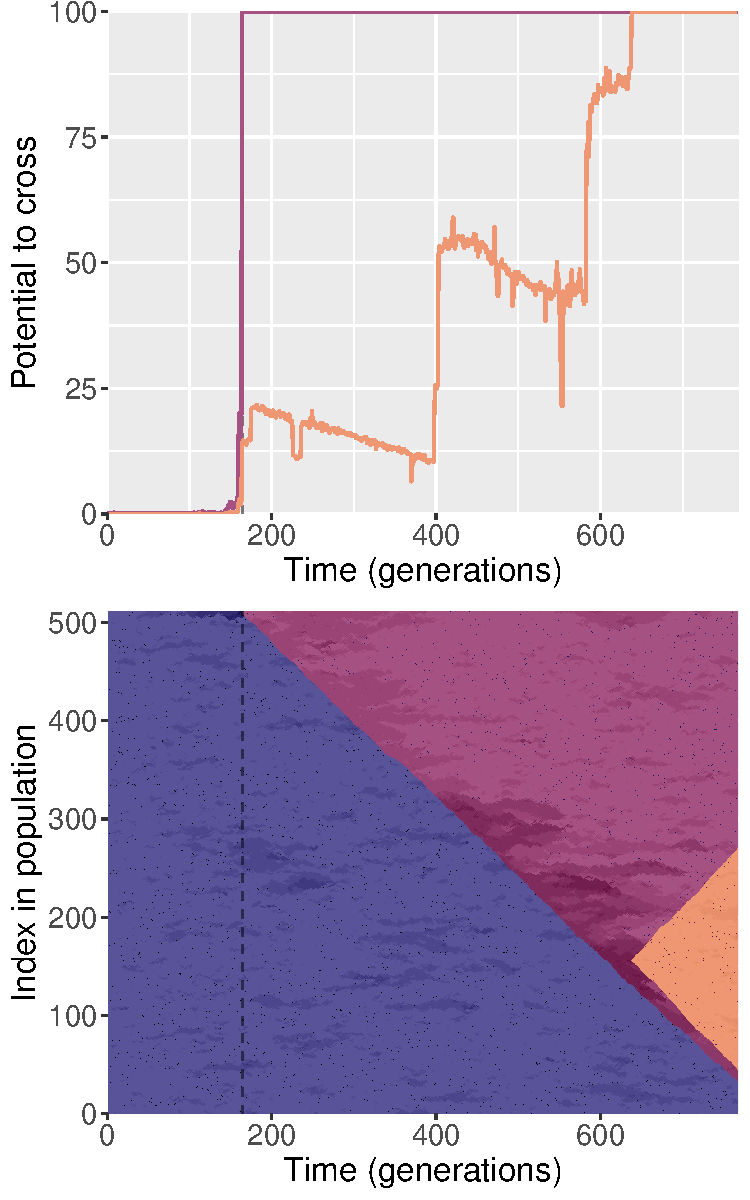
\includegraphics[width=0.6\textwidth]{05_adaptive_momentum/media/reps/no_am_two_cross/script_06__plot_02__combined_plot.pdf}
% \caption{
%     \textbf{Top plot}: The analytic replay data for a representative replicate that did \textit{not} start in a momentum window but still managed to cross a valley. 
%     The red line shows the potential to cross the first valley, while the orange line shows the potential to cross the second valley. 
%     \textbf{Bottom plot}: a Muller plot of the original population, like in Figure \ref{fig-replay-single-cross}.
% }
% \label{fig-replay-no-window}
% \end{center}
% \end{figure}

% Finally, we also show the potentiation of crossing the second valley, which in some cases is realized (as in Figures \ref{fig-replay-double-cross} and \ref{fig-replay-no-window}), and other times is not (Figures \ref{fig-replay-single-cross} and \ref{fig-replay-no-cross}).
% As potentiation is probabilistic in nature, the potential to cross the second valley can be thought of as the product of crossing the first valley from the current state of the population and the probability of crossing a second valley from a naive starting position (i.e, the elevated potentiation of a population at the beginning of a sweep). 
% We see this dynamic reflected early in the replays -- increases in first-cross potential are reflected, at much smaller scales, in second-cross potential. 
% Once the first valley is crossed, the potential to cross the second valley can increase dramatically. 
% We see sizable increases in second-cross potential upon successful crossing of the first valley in Figures \ref{fig-replay-single-cross} and \ref{fig-replay-double-cross}. %, \ref{fig-replay-no-window}, and . 
% This result is consistent with adaptive momentum framework, which posits that the discovery of a new peak will initiate a new adaptive momentum window. 
% Most strikingly, this same dynamic holds true for Figure \ref{fig-replay-no-window} -- while the replicate did not start in a momentum window, we see the first cross create a window and the potential of the second cross reflects that.

% \subsection{Shuffled population experiments}

% To test the effect of population structure on potentiation, we repeated the benchmarking and replay experiments with shuffled populations. 
% In both cases, the experiments were repeated exactly, except for one additional shuffle step: before beginning to evolve the populations, we would shuffle the order of organisms in the population, and then proceed with evolution as normal. 
% %We replayed the evolution of 10 randomly-sampled single-cross replicates, and 

% The shuffled benchmark data in Figure \ref{fig-combined-plots}C shows that only populations with a leading edge of $p_{2} + 5$ are able to maintain greater than a 10\% chance to cross if the leading edge has swept more than half the population.
% Two differences arise when we shuffle the benchmark populations that can decrease crossing potential: 
% 1) fixation can occur faster because of multiple leading edges and 
% 2) when the eight organisms from the leading edge are shuffled into the population, they are likely to be purified faster.
% %When the benchmark populations are shuffled, fixation occurs more rapidly and thus the potential to cross falls quickly.  

% A representative sample from the 10 single-cross replicates is shown in Figure \ref{fig-replay-shuffle}. 
% The replay data indicate that potential to cross remains relatively low, never reaching a 20\% chance, until a critical mass of nearly-crossed organisms skyrockets the potential from 9.2\% to 100\%. 
% The earlier spikes in potentiation always correspond to the appearance of a single organism that is one step away from crossing the valley, which was then lost in the original population.
% These trends were consistent across all 10 replicates that were replayed \citep{austin_ferguson_2024_11507982}. 

% \begin{figure}[h!]
% \begin{center}
% 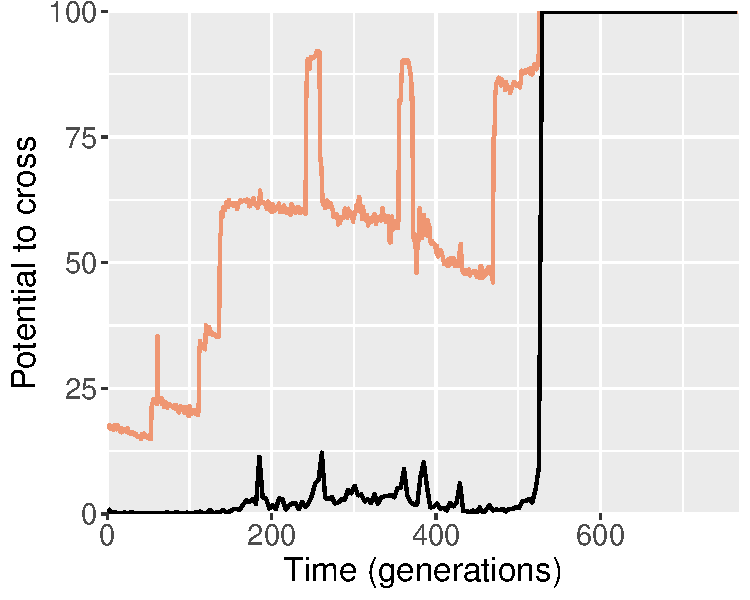
\includegraphics[width=0.6\textwidth]{05_adaptive_momentum/media/reps/400/script_07__plot_01__selected_replays_with_shuffled_replays_no_bg.pdf}
% \caption{
%     The black line (bottom) shows the potential for a shuffled population to cross a valley. 
%     The orange line (top) shows the standard potential for the population to cross (same data as Figure \ref{fig-replay-single-cross}). 
%     The shuffled line consists of 1,000 samples every 4 generations. 
%     %Background shading shows the expected potential to cross when an idealized leading edge population is shuffled (a shuffled version of Figure \ref{fig-benchmarking}). 
% }
% \label{fig-replay-shuffle}
% \end{center}
% \end{figure}

% % \begin{figure}[h!]
% % \begin{center}
% % 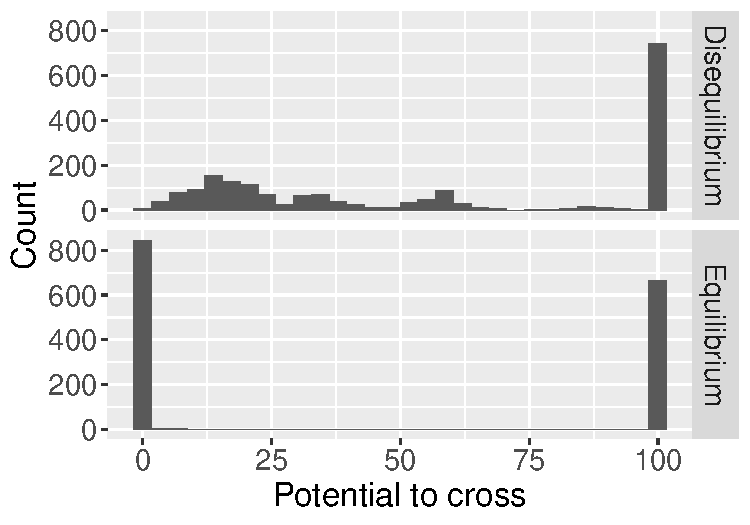
\includegraphics[width=0.45\textwidth]{media/combined_potentiation_histograms.pdf}
% % \caption{
% %     Histogram of potentiation values in replicates in a momentum window (disequilibrium, top) and outside a window (equilibrium, bottom).
% % }
% % \label{fig-histograms}
% % \end{center}
% % \end{figure}
